% nn-one-two.png -- the two small networks of sections 3 and 4, side by side:
%   (a) one_neuron   = Linear(1,1) -> Sigmoid -> Linear(1,1), 4 parameters
%   (b) two_neurons  = Linear(1,2) -> Sigmoid -> Linear(2,1), 6 parameters
% The weight labels are the names used by the printout in the notebook.
% Build: bash tools/figures/build.sh
\documentclass[tikz,border=5pt]{standalone}
% Shared style for the neural-network diagrams in notebooks/img/nn-*.png.
% Palette and look are matched to the pre-existing figures (nn-1..nn-8,
% backprop-*) so a regenerated figure sits next to them unnoticed.
\usepackage[T1]{fontenc}
\usepackage{newtxtext}
\usepackage{newtxmath}
\usetikzlibrary{arrows.meta,calc,positioning}

\definecolor{innavy}{HTML}{004475}     % input neurons, source-like labels
\definecolor{hidyellow}{HTML}{FFCF6E}  % hidden neurons
\definecolor{outmaroon}{HTML}{8E1854}  % output neuron
\definecolor{accgold}{HTML}{E5A600}    % "Hidden Layer" label
\definecolor{gridgrey}{HTML}{B7B7B7}

\tikzset{
  neuron/.style   = {circle, draw=black, line width=0.9pt, minimum size=0.9cm,
                     inner sep=0pt, font=\large\bfseries},
  hidden/.style   = {neuron, fill=hidyellow},
  inputn/.style   = {neuron, fill=innavy, text=white},
  outputn/.style  = {neuron, fill=outmaroon, text=white},
  conn/.style     = {-{Latex[length=2.2mm,width=1.6mm]}, line width=0.7pt},
  bias/.style     = {-{Latex[length=1.8mm,width=1.3mm]}, line width=0.7pt},
  biaslbl/.style  = {font=\scriptsize, inner sep=1pt},
  layerlbl/.style = {font=\large\bfseries},
}

% Column positions shared by every figure (1 unit = 1cm).
\def\HIDX{3.4}   % hidden neurons
\def\ACTX{4.9}   % activation insets (centre)
\def\OUTX{7.4}   % output neuron
\def\NODE{0.45}  % neuron radius
\def\BOX{0.42}   % activation inset half-width

% Framed mini-plot of the sigmoid, drawn where the existing figures draw it.
% Usage: \actinset{x}{y}{label}
\newcommand{\actinset}[3]{%
  \begin{scope}[shift={(#1,#2)}]
    \fill[white] (-\BOX,-\BOX) rectangle (\BOX,\BOX);
    \foreach \g in {-0.14,0.14}{%
      \draw[gridgrey, line width=0.35pt] (-\BOX,\g) -- (\BOX,\g);
      \draw[gridgrey, line width=0.35pt] (\g,-\BOX) -- (\g,\BOX);}
    \draw[black, line width=1.1pt, domain=-0.40:0.40, samples=60]
      plot ({\x}, {0.78/(1+exp(-9*\x)) - 0.39});
    \draw[black, line width=0.9pt] (-\BOX,-\BOX) rectangle (\BOX,\BOX);
    \node[above left, font=\scriptsize, inner sep=1pt] at (\BOX,\BOX+0.02) {#3};
  \end{scope}}

% Bias arrow plus label above a neuron: \biasup{node name}
\newcommand{\biasup}[1]{%
  \draw[bias] ($(#1)+(0,\NODE+0.41)$) -- ($(#1)+(0,\NODE+0.01)$);
  \node[biaslbl, above] at ($(#1)+(0,\NODE+0.41)$) {Bias};}

% A vector collapsed into one node: two offset discs behind it.
% Usage: \vectornode{x}{y}{label}
\newcommand{\vectornode}[3]{%
  \foreach \dx/\dy in {0.13/0.11, 0.26/0.22}{%
    \draw[innavy, line width=0.7pt, fill=innavy!22]
      ($(#1,#2)+(\dx,\dy)$) circle (\NODE);}
  \node[inputn] (#3) at (#1,#2) {$#3$};}

\begin{document}
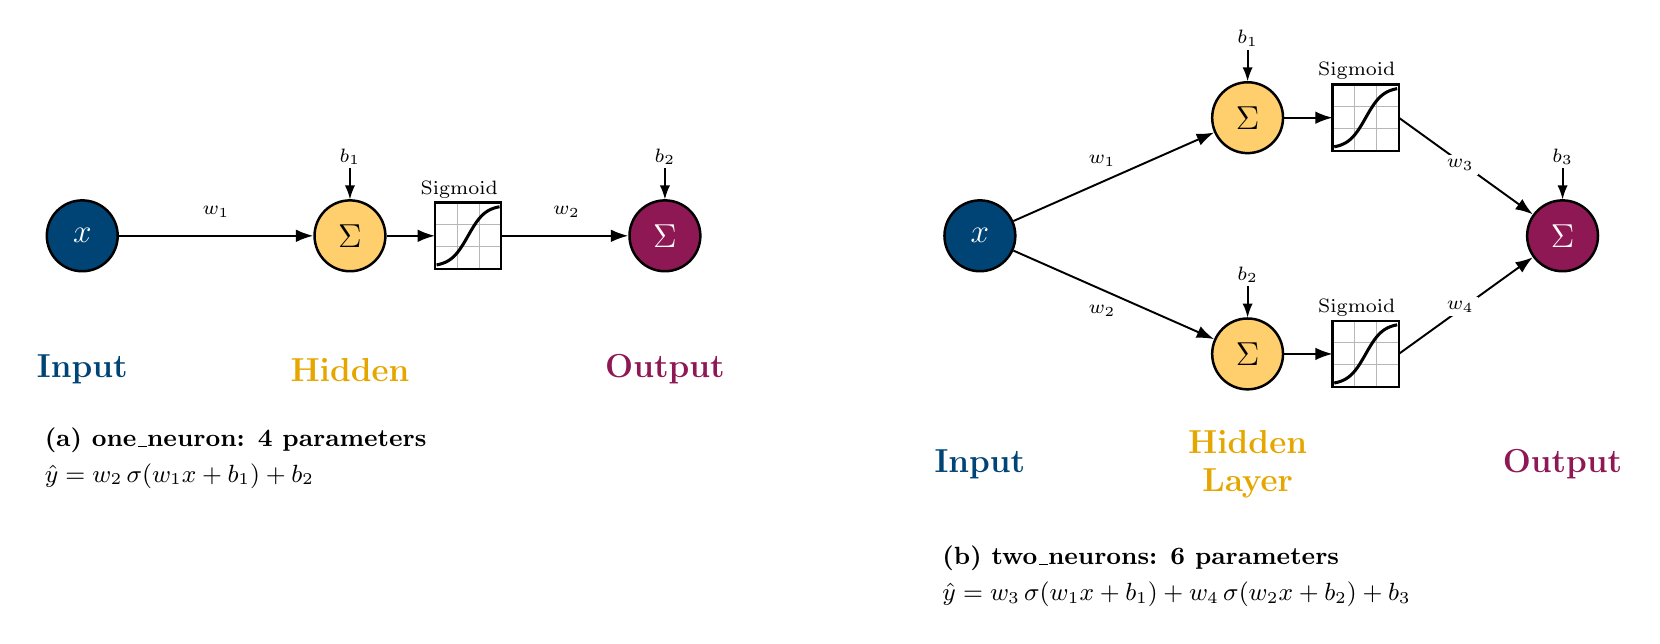
\begin{tikzpicture}[x=1cm,y=1cm]

% bias arrow with a parameter name instead of the generic "Bias"
\newcommand{\biasp}[2]{%
  \draw[bias] ($(#1)+(0,\NODE+0.41)$) -- ($(#1)+(0,\NODE+0.01)$);
  \node[biaslbl, above] at ($(#1)+(0,\NODE+0.41)$) {$#2$};}
% weight label sitting on a connection, with a white background
\tikzset{wlab/.style={font=\scriptsize, inner sep=1.5pt, fill=white}}

% =====================================================================
% (a) one sigmoid neuron with a linear read-out
% =====================================================================
\begin{scope}
  \node[inputn] (x) at (0,0) {$x$};
  \node[hidden] (h) at (\HIDX,0) {$\Sigma$};
  \actinset{\ACTX}{0}{Sigmoid}
  \node[outputn] (o) at (\OUTX,0) {$\Sigma$};

  \draw[conn] (x) -- (h);
  \draw[conn] (h) -- (\ACTX-\BOX,0);
  \draw[conn] (\ACTX+\BOX,0) -- (o);
  \biasp{h}{b_1}
  \biasp{o}{b_2}

  \node[wlab] at (1.7,0.30) {$w_1$};
  \node[wlab] at (6.15,0.30) {$w_2$};

  \node[layerlbl, text=innavy,    align=center] at (0,-1.7)     {Input};
  \node[layerlbl, text=accgold,   align=center] at (\HIDX,-1.7) {Hidden};
  \node[layerlbl, text=outmaroon, align=center] at (\OUTX,-1.7) {Output};

  \node[font=\small\bfseries, anchor=west, align=left] at (-0.6,-2.6)
    {(a) one\_neuron: 4 parameters};
  \node[font=\small, anchor=west] at (-0.6,-3.05)
    {$\hat y=w_2\,\sigma(w_1x+b_1)+b_2$};
\end{scope}

% =====================================================================
% (b) one hidden layer with two neurons
% =====================================================================
\begin{scope}[xshift=11.4cm]
  \node[inputn] (x) at (0,0) {$x$};
  \foreach \j/\yy in {1/1.5, 2/-1.5}{%
    \node[hidden] (h\j) at (\HIDX,\yy) {$\Sigma$};
    \actinset{\ACTX}{\yy}{Sigmoid}
    \draw[conn] (h\j) -- (\ACTX-\BOX,\yy);
    \biasp{h\j}{b_\j}}
  \node[outputn] (o) at (\OUTX,0) {$\Sigma$};
  \biasp{o}{b_3}

  \foreach \j in {1,2}{\draw[conn] (x) -- (h\j);}
  \foreach \yy in {1.5,-1.5}{\draw[conn] (\ACTX+\BOX,\yy) -- (o);}

  \node[wlab] at (1.55,0.95)  {$w_1$};
  \node[wlab] at (1.55,-0.95) {$w_2$};
  \node[wlab] at (6.10,0.90)  {$w_3$};
  \node[wlab] at (6.10,-0.90) {$w_4$};

  \node[layerlbl, text=innavy,    align=center] at (0,-2.9)     {Input};
  \node[layerlbl, text=accgold,   align=center] at (\HIDX,-2.9) {Hidden\\Layer};
  \node[layerlbl, text=outmaroon, align=center] at (\OUTX,-2.9) {Output};

  \node[font=\small\bfseries, anchor=west, align=left] at (-0.6,-4.1)
    {(b) two\_neurons: 6 parameters};
  \node[font=\small, anchor=west] at (-0.6,-4.55)
    {$\hat y=w_3\,\sigma(w_1x+b_1)+w_4\,\sigma(w_2x+b_2)+b_3$};
\end{scope}

\end{tikzpicture}
\end{document}
